\section[Cote 64 : la configuration octaédrale en caractéristique 5]{Cote 64 : la configuration octaédrale en caractéristique 5\protect\verifie{Folder64}}\label{sec:64}

La cote 64, \emph{Modules courbes elliptiques en caractéristiques $\neq 2$ : notes manuscrites (s.d.)}, cent cinquante-six pages que l'inventaire date \q{[à partir de 1980-1982]}, consacre sa partie~II aux structures octaédrales dans $\mathbf P^1$ (pages~43 à~52, \lot{64}{3}{44}). Une action fidèle du groupe de Klein se met localement sous la forme $\sigma_1(z) = -z$, $\sigma_2(z) = 1/z$, et la somme des axes est la configuration octaédrale $\Delta = \{0, \infty, \pm 1, \pm i\}$. Pour identifier $\mathrm{Aut}(X, \Delta)$ au groupe des rotations de l'octaèdre, la page~48 calcule le fixateur de deux sommets non opposés, $\infty$ et $-1$ : un tel automorphisme s'écrit $z \mapsto az + (a - 1)$, et s'il n'est pas l'identité il permute $\{0, 1, i, -i\}$. Les quatre conditions sur $a$ qui en résultent ont, dit la page, une intersection vide hors des caractéristiques $2$ et~$5$. La marge borne le calcul par \q{car.\ $\neq 3$ et $5$}, et la lecture ajoute l'hypothèse \q{$5$ inversible} partout où elle sert.

\begin{theoreme}[Grothendieck, page 48]\label{thm:64-fixateur}
Soit $K$ un corps où $2 \neq 0$, et $i \in K$ avec $i^2 = -1$. Si $z \mapsto az + (a - 1)$ envoie $\{0, 1, i, -i\}$ dans lui-même, alors $5(a - 1) = 0$. En particulier, si $5 \neq 0$ dans $K$, le fixateur de $\infty$ et $-1$ dans $\mathrm{Aut}(\mathbf P^1_K, \Delta)$ est trivial.
\end{theoreme}

\begin{proof}
Les quatre points sont distincts, puisque $2 \neq 0$. Si $a = 0$, l'image de $0$ est $-1$, qui n'est aucun des quatre points. Sinon l'application est injective, donc permute les quatre points, et conserve leur somme, qui vaut~$1$ ; or elle la change en $a \cdot 1 + 4(a - 1) = 5a - 4$. D'où $5(a - 1) = 0$.
\end{proof}

Les six points de $\Delta$ sont les sommets d'un octaèdre dont les sommets opposés sont $0$ et $\infty$, $1$ et $-1$, $i$ et $-i$. Le fixateur de deux sommets non opposés, $\infty$ et $-1$ (cerclés), permute les quatre autres.
\begin{center}
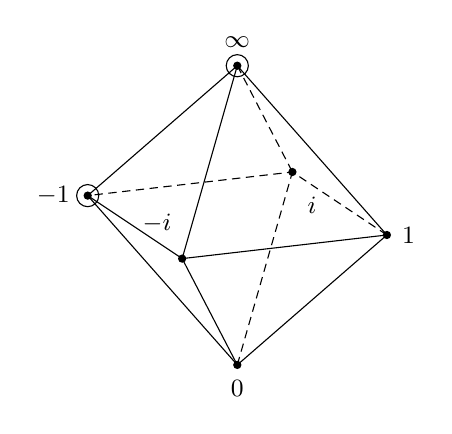
\begin{tikzpicture}[x=1cm, y=1cm, every node/.style={font=\small}]
\coordinate (inf) at (0,1.9); \coordinate (z) at (0,-1.9);
\coordinate (p1) at (1.9,-0.25); \coordinate (m1) at (-1.9,0.25);
\coordinate (pi) at (0.7,0.55); \coordinate (mi) at (-0.7,-0.55);
\draw (m1)--(mi)--(p1); \draw[densely dashed] (p1)--(pi)--(m1);
\foreach \v in {m1,mi,p1} { \draw (inf)--(\v); \draw (z)--(\v); }
\draw[densely dashed] (inf)--(pi); \draw[densely dashed] (z)--(pi);
\foreach \v in {inf,z,p1,m1,pi,mi} \fill (\v) circle (1.5pt);
\draw (inf) circle (4pt); \draw (m1) circle (4pt);
\node[above=3pt] at (inf) {$\infty$}; \node[below=2pt] at (z) {$0$};
\node[right=2pt] at (p1) {$1$}; \node[left=3pt] at (m1) {$-1$};
\node at (0.95,0.13) {$i$}; \node at (-1.02,-0.1) {$-i$};
\end{tikzpicture}
\end{center}

\begin{contrexemple}[énoncé de l'édition, d'après la note de la lecture à la page 49]\label{ce:64-car5}
En caractéristique~$5$, le fixateur de $\infty$ et $-1$ n'est pas trivial : $z \mapsto 2z + 1$ permute $\{0, 1, i, -i\}$. Sur $\mathbf F_5$, avec $i = 2$, la configuration $\Delta$ est $\mathbf P^1(\mathbf F_5)$ tout entier ; les bijections de $\mathbf P^1(\mathbf F_5)$ induites par $\mathrm{GL}_2(\mathbf F_5)$, qui préservent toutes $\Delta$, sont au nombre de $120$ et non de $24$, et le fixateur de $\infty$ et $-1$ est formé de l'identité et des $z \mapsto az + (a - 1)$ pour $a = 2, 3, 4$.
\end{contrexemple}

\begin{proof}
Comme $i^2 = -1 = 4$, $i = \pm 2$. Pour $i = 2$, l'application $z \mapsto 2z + 1$ envoie $0 \mapsto 1 \mapsto 3 = -i \mapsto 2 = i \mapsto 0$ ; de même pour $i = -2$. Sur $\mathbf F_5$, les six points $\infty, 0, 1, -1, 2, -2$ sont les six points de $\mathbf P^1(\mathbf F_5)$. Le décompte des bijections induites et du fixateur se fait sur les $625$ matrices de $M_2(\mathbf F_5)$ ; Lean le vérifie par calcul (\texttt{card\_pgl}, \texttt{card\_fixer}).
\end{proof}

\begin{remarque}
La démonstration du théorème~\ref{thm:64-fixateur} n'utilise que $2 \neq 0$ et $5 \neq 0$ : la caractéristique~$3$, que la marge exclut, n'a pas à l'être. Le contre-exemple confirme l'hypothèse \q{$5$ inversible} de la lecture : sans elle, $\mathrm{Aut}(X, \Delta)$ est $\mathrm{PGL}_2(\mathbf F_5)$, d'ordre $120$, et non le groupe des rotations de l'octaèdre, d'ordre~$24$.
\end{remarque}

Ne sont pas démontrés ici : la forme normale locale de la page~46, l'égalité $\mathrm{Aut}(X, \Delta) = \mathrm{Aut}^+_{\mathrm{oct}}(\Delta)$ qui suit du théorème, et les énoncés relatifs au-dessus d'une base, qui restent ouverts :

\begin{encadre}
\begin{theoreme*}[Grothendieck, pages 44 à 52, configurations octaédrales sur une base ; voir aussi Beauville~\cite{beauville2010}\piste{64-octahedral-configurations-relative}]\nonverifie
Soit $X$ un fibré en droites projectives sur un schéma $S$ de caractéristiques résiduelles différentes de~$2$. Se correspondent bijectivement : les sous-schémas en groupes de $\mathrm{Aut}_S(X)$ localement isomorphes à $(\mathbf Z/2)^2$, ceux localement isomorphes à $\mathfrak S_4$, et les configurations octaédrales régulières, diviseurs étales de degré~$6$ munis d'une antipodie. Les couples $(X, \Delta)$ dont le torseur d'orientation est identifié à $\mu_4^*$ équivalent aux revêtements étales finis de degré~$4$ de~$S$.
\end{theoreme*}
\end{encadre}
{\small Les feuillets en esquissent une démonstration incomplète (pages 46 à 49). Le corollaire~2 n'est pas démontré, et l'hypothèse qui en fait une équivalence est une addition marginale de lecture incertaine. Là où la page identifie $\mathrm{Aut}_S(X, \Delta)$ au groupe des rotations de l'octaèdre, l'édition suppose $5$ inversible, hypothèse nécessaire par le contre-exemple~\ref{ce:64-car5}. Beauville traite le cas d'un corps, sans base. Mathlib n'a pas les formes de $\mathbf P^1$ sur une base.\par}

\begin{encadre}
\begin{theoreme*}[Grothendieck, pages 74 à 79 et 84 à 91, épinglages de Legendre ; voir aussi Antieau--Meier~\cite{antieaumeier2020}\piste{64-legendre-pinning-moduli}]\nonverifie
Sur $\mathbf Z[1/2]$, les courbes elliptiques munies d'un épinglage de Jacobi de niveau~$2$ et d'un épinglage de Legendre (un vecteur tangent à l'origine, tordu par un $\mu_4$-torseur fixé, dont le carré correspond à l'espace tangent de $E/\pm1$ en l'image de l'origine) forment un groupoïde rigide représenté par $U_{0,3} \times \mu_4^*$. Le groupe $\mu_4 \times \mathfrak S_3$ opère sur ce schéma, $\mathfrak S_3$ tautologiquement sur $U_{0,3}$ et par la signature sur~$\mu_4^*$.
\end{theoreme*}
\end{encadre}
{\small La représentabilité est affirmée sans démonstration (page~85). Antieau et Meier (2020, définition~4.4, proposition~4.5 et lemme~4.7 dans la numérotation de arXiv:1608.00851) décrivent, sur $\mathbf Z[1/2]$, l'espace de Legendre $X = \mathbf A^1 \smallsetminus \{0, 1\}$ comme le $C_2$-torseur des racines carrées de $p\,\omega^{\otimes 2}$ au-dessus de $\mathcal M(2) \simeq BC_{2,X}$, et notent que l'action de $\mathfrak S_3$ ne se relève pas strictement à $X$ ; l'épinglage tordu par $\mu_4^*$, qui rend l'action de $\mu_4 \times \mathfrak S_3$ stricte sur $U_{0,3} \times \mu_4^*$, n'y figure pas. Le $\mathfrak S_3$ qui opère ici sur $U_{0,3}$ est celui des sections~\ref{sec:62} et~\ref{sec:146}. Mathlib n'a pas les espaces de modules de courbes elliptiques. On se reportera aux notes de Grothendieck (\lot{64}{4}{74}).\par}
